\documentclass{article}
\usepackage{mathtools}
\usepackage{amsmath}
\usepackage{amssymb}
\usepackage{tikz}

\begin{document}
	
	\title{MAT11001 – Harjoitus 1}
	\date{}
	\maketitle
	
	
	\section*{Tehtävä 1}

	
\begin{enumerate}


	\item[(a)]
	\[
	\pi \notin \mathbb{Q}
	\]	
	
	\item[(b)]
	\[
	\{-5, 1, 27, 100\} \subset \mathbb{Z}
	\]

	\item[(c)]
	\[
	C \neq \emptyset \quad \text{ja} \quad C \subset A \setminus B
	\]

	\item[(d)]
	\[
	\{ x \in \mathbb{R} \mid  \sqrt[3]{x} \geq -0,123 \ \text{ja} \  \sqrt[3]{x} \leq 1,234 \}
	\]

	\item[(e)]
	\[
	p \in \mathbb{Q} \ \text{ja} \ q \in \mathbb{Q} \implies p + q \in \mathbb{Q}
	\]

	\item[(f)]
	\[
	\{b\} \cup B \subset \complement A
	\]

	\item[(g)]
	\[
	\{n \in \mathbb{N} \mid n > 1 \mid \exists a, b \in \mathbb{N}, \ 1 < a < n, \ 1 < b < n, \ a \cdot b = n \} 
	\]

	\item[(h)]
	\[
	\{ x \in \mathbb{R} \mid x \in [1, 3]\} \cap \{ y \in \mathbb{R} \mid y \in ]2, 4[\} = \{ z \in \mathbb{R} \mid z \in [2, 3[\}
	\]

	
\end{enumerate}




\newpage

	\section*{Tehtävä 2}

	\( $A = \{1, 2, 3, 4, 5, 6\}$ \ \text{ja} \ $B = \{2, 4, 6, 8\}$\)

\begin{enumerate}

	\item[(a)]
	\[
	A \cup B = \{1, 2, 3, 4, 5, 6, 8\}
	\]
	\[
	A \cap B = \{2, 4, 6\}
	\]

	\item[(b)]
	\[
	A \setminus B = \{ 1, 3, 5\}
	\]
	\[
	B \setminus A = \{ 8\}
	\]

	\item[(c)]
	\[
	A \Delta B = A \setminus B \cup B \setminus A = \{1, 3, 5, 8\}
	\]
	
	\item[(d)]
		
	\[
	\begin{aligned}
	P(B) = \{ &\emptyset, \{2\}, \{4\}, \{6\}, \{8\}, B\} \\
	= \{ 
		&\emptyset, \{ 2 \}, \{ 4 \}, \{ 6 \}, \{ 8 \}, \\
		&\{ 2, 4 \}, \{ 2, 6 \}, \{ 2, 8 \}, \{ 4, 6 \}, \{ 4, 8 \}, \\
		&\{ 2, 4, 6 \}, \{ 2, 4, 8 \}, \{ 2, 6, 8 \}, \{ 4, 6, 8 \}, \\
		&\{ 2, 4, 6, 8 \}
	  \}
	\end{aligned}
	\]
		
\end{enumerate}


\newpage

\section*{Tehtävä 3}

\begin{enumerate}
	
	\item[(a)]
	\[
	\{1/n^{2}: \ n \in \mathbb{P} \ \text{ja} \  n < 13 \} = \{ \frac{1}{4}, \frac{1}{9}, \frac{1}{25}, \frac{1}{49}, \frac{1}{121} \}
	\]

	\item[(b)]
	\[
	\{ 2+ (-1)^{n}: n \in \mathbb{N}\} = \{ 1, 3 \}
	\]

	\item[(c)]
	\[
	\begin{aligned}
	&\{x \in \mathbb{R}: x^{2} - 4x  + 2 = 0\} \\
	\\
	&\text{Ratkaistaan toisen asteen yhtälö:} \\
	&x = \frac{-b \pm\sqrt{b^2 - 4ac}}{2a}, \quad \text{missä} \ a = 1, b = -4, c = 2 \\
	\implies &x = \frac{4 \pm \sqrt{8}}{2} = 2 \pm \sqrt{2} \\
	\implies &\{x \in \mathbb{R}: x^{2} - 4x + 2 = 0\} = \{2 - \sqrt{2}, 2 + \sqrt{2}\}
	\end{aligned}
	\]

	\item[(d)]
	\[
	\{z \in \mathbb{Z}: \sqrt{\lvert z \rvert} < 1 \frac{1}{2} \} = \{ -2, -1, 0, 1, 2 \}
	\]

	\item[(e)]
	\[
	\begin{aligned}
	&\{x \in \mathbb{Q}: x^{2} = 2\} \\
	\\
	&\text{Ratkaistaan toisen asteen yhtälö:} \\
	&x = \frac{-b \pm\sqrt{b^2 - 4ac}}{2a}, \quad \text{missä} \ a = 1, b = 0, c = -2 \\
	\implies &x = \frac{\pm \sqrt{8}}{2} = \pm \sqrt{2} \\	
	\\ &\text{Koska kahden neliöjuuri ei ole rationaaliluku:} \\
	\implies &\{x \in \mathbb{Q}: x^{2} = 2\} = \emptyset
	\end{aligned}
	\]

\end{enumerate}


\newpage

\section*{Tehtävä 4}

Osoita, että 893 ei ole alkuluku.

\begin{flushleft}
Tarkistetaan, onko 893 jaollinen pienillä alkuluvuilla (enintään \( \sqrt{893} \approx 29.9 \)).
\end{flushleft}

\begin{itemize}
	\item \textbf{2:} 893 on pariton, joten se ei ole jaollinen 2:lla.
	\item \textbf{3:} Lasketaan \(893 \div 3 = 297.666\ldots\). Koska tulos ei ole kokonaisluku, 893 ei ole jaollinen 3:lla.
	\item \textbf{5:} Luku ei pääty 0:aan tai 5:een, joten se ei ole jaollinen 5:llä.
	\item \textbf{7:} Lasketaan \(893 \div 7 \approx 127.57\), joka ei ole kokonaisluku. Siten 893 ei ole jaollinen 7:llä.
	\item \textbf{11, 13, 17, 19, 23, 29:} Kokeillaan nämä yksitellen.
\end{itemize}

\begin{flushleft}
Kokeillaan lukua 19:
\end{flushleft}
\[
893 \div 19 = 47.
\]

\begin{flushleft}
Luku 47 on kokonaisluku, joten 893 voidaan esittää tulona:
\end{flushleft}
\[
893 = 19 \times 47.
\]

\begin{flushleft}
Koska 893 voidaan jakaa luvuilla 19 ja 47 (molemmat ovat alkulukuja), sillä on muitakin jakajia kuin 1 ja 893 itse.
\end{flushleft}

\begin{flushleft}
\textbf{Johtopäätös:} Luku 893 ei ole alkuluku.
\end{flushleft}


\newpage

\section*{Tehtävä 5}

Olkoot \(A \subset X \text{ ja } B \subset X\)

\begin{enumerate}
	
\item[(a)]

Osoitetaan, että
\[
(A \cup B) \cap \complement A \subset B.
\]

Olkoon \(x \in (A \cup B) \cap \complement A\).

Tällöin \(x \in (A \cup B)\) ja \(x \in \complement A\).

\begin{itemize}
	\item \(x \in (A \cup B)\) tarkoittaa, että \(x \in A\) tai \(x \in B\).
	\item \(x \in \complement A\) tarkoittaa, että \(x \notin A\).
\end{itemize}

Näin ollen \(x \notin A\) ja \(x \in (A \cup B)\), mikä tarkoittaa, että \(x \in B\).

Tästä seuraa, että \(x \in B\), ja siis

\[
(A \cup B) \cap \complement A \subset B.
\]


\item[(b)]
4b - Venn Diagrammi

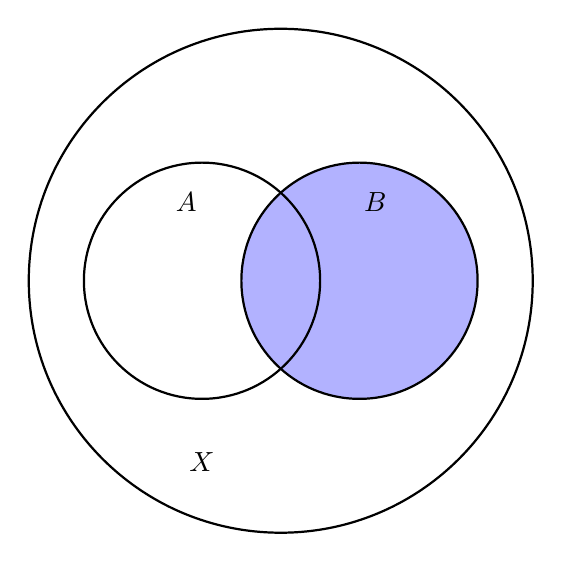
\begin{tikzpicture}
	% Universumi X
	\draw[thick] (0,0) circle (3.2);  % Piirrä universumi X
	
	% Joukkojen A ja B yhdiste varjostettuna (A ∪ B)
	\begin{scope}
		\clip (-1,0) circle (1.5);  % Leikkaa joukon A alue
		\fill[gray!30] (1,0) circle (1.5);  % Täytä joukko B (A ∪ B)
	\end{scope}
	
	% Komplementti A ja B yhteisalue varjostettuna ((A ∪ B) ∩ ¬A)
	\begin{scope}
		\clip (1,0) circle (1.5);  % Leikkaa joukon B alue
		\fill[blue!30] (-3,-2) rectangle (3,2);  % Täytä alue ¬A
	\end{scope}
	
	% Joukko A
	\draw[thick] (-1,0) circle (1.5);
	\node at (-1.2, 1) {$A$};  % Nimeä joukko A
	
	% Joukko B
	\draw[thick] (1,0) circle (1.5);
	\node at (1.2, 1) {$B$};  % Nimeä joukko B
	
	% Universumi X
	\node at (-1.0, -2.3) {$X$};  % Nimeä universumi X
\end{tikzpicture}

\end{enumerate}


\newpage

\section*{Tehtävä 6}

Testipalautus..

\end{document}